%\documentclass[12pt,preprint]{aastex}
\documentclass[iop,apj]{emulateapj}
%\usepackage{multirow}
\usepackage{longtable}
\usepackage{ulem}
%\usepackage[monochrome]{color}
\usepackage{color}
%\usepackage{lipsum}
\usepackage{amsmath}
%\usepackage{hyperref}

\newcommand{\eqqref}[1]{Equation (\ref{#1})}
\newcommand{\tabref}[1]{Table~\ref{#1}}
\newcommand{\figref}[1]{Figure~\ref{#1}}
\newcommand{\secref}[1]{Section~\ref{#1}}
\newcommand{\appref}[1]{Appendix~\ref{#1}}

\newcommand{\SNeIa}{SNe~Ia}
\newcommand{\SNIa}{SN~Ia}
\newcommand{\C}[1]{\ensuremath{{}^{#1}{\rm C}}}
\newcommand{\Ox}[1]{\ensuremath{{}^{#1}{\rm O}}}
\newcommand{\Ne}[1]{\ensuremath{{}^{#1}{\rm Ne}}}
\newcommand{\Na}[1]{\ensuremath{{}^{#1}{\rm Na}}}
\newcommand{\Mg}[1]{\ensuremath{{}^{#1}{\rm Mg}}}
\newcommand{\Ni}[1]{\ensuremath{{}^{#1}{\rm Ni}}}
\newcommand{\Co}[1]{\ensuremath{{}^{#1}{\rm Co}}}
\newcommand{\Si}[1]{\ensuremath{{}^{#1}{\rm Si}}}
\newcommand{\Fe}[1]{\ensuremath{{}^{#1}{\rm Fe}}}
\newcommand{\code}[1]{\textsc{#1}}
\newcommand{\FLASH}{\code{FLASH}}
\newcommand{\CASTRO}{\code{CASTRO}}
\newcommand{\MESA}{\code{MESA}}
\newcommand{\PARAMESH}{\code{PARAMESH}}
\newcommand{\pv}{\ensuremath{\phi}}
\newcommand{\bvec}[1]{\ensuremath{\boldsymbol{#1}}} %boldface vector style
\newcommand{\grad}{\bvec{\nabla}} %gradient
\newcommand{\curl}{\bvec{\nabla \times}} %curl
\newcommand{\Atwood}{\ensuremath{\mathrm{At}}}
\newcommand{\adndt}{At.~Data~Nucl.~Data~Tables}
\newcommand{\At}{{\rm At}}
\newcommand{\ee}[1]{\ensuremath{\times 10^{#1}}}
\newcommand{\cdens}{\rho_{c}}

% basic unit typesetteing
\newcommand{\unitspace}{\ensuremath{\,}}
\newcommand{\usp}{\unitspace}
\newcommand{\numberspace}{\ensuremath{\;}}
\newcommand{\nsp}{\numberspace}
\newcommand{\unitstyle}[1]{\ensuremath{\mathrm{#1}}}
\newcommand{\power}[2]{\ensuremath{{#1}^{#2}}}


% prefixes
\newcommand{\nano}{\unitstyle{n}}
\newcommand{\milli}{\unitstyle{m}}
\newcommand{\centi}{\unitstyle{c}}
\newcommand{\kilo}{\unitstyle{k}}
\newcommand{\Mega}{\unitstyle{M}}
\newcommand{\Giga}{\unitstyle{G}}

% base units, mks
\newcommand{\meter}{\unitstyle{m}}
\newcommand{\kilogram}{\kilo\gram}
\newcommand{\second}{\unitstyle{s}}

\newcommand{\Kelvin}{\unitstyle{K}}
\newcommand{\K}{\Kelvin}  %degrees Kelvin


% base units, cgs
\newcommand{\cm}{\centi\meter}
\newcommand{\gram}{\unitstyle{g}}


% derived units
\newcommand{\grampercc}{\gram\usp\power{\cm}{-3}} %mass density
\newcommand{\grampersquarecm}{\gram\usp\power{\cm}{-2}} %column depth
\newcommand{\GramPerCc}{\grampercc}
\newcommand{\GramPerSc}{\grampersquarecm}
\newcommand{\columnunit}{\grampersquarecm}
\newcommand{\dyne}{\unitstyle{dyn}} %dyne
\newcommand{\erg}{\unitstyle{ergs}} %ergs
\newcommand{\ergs}{\erg}
\newcommand{\gauss}{\unitstyle{G}} %gauss
\newcommand{\ergspersecond}{\erg\unitspace\power{\second}{-1}}
\newcommand{\ergspergram}{\erg\unitspace\power{\gram}{-1}}
\newcommand{\cgsflux}{\erg\unitspace\power{\cm}{-2}\usp\power{\second}{-1}}
\newcommand{\kms}{\kilo\meter\unitspace\power{\second}{-1}}

% Nuclear and atomic units
\newcommand{\amu}{\unitstyle{u}} %atomic mass unit
\newcommand{\angstrom}{\mbox{\AA}} %Angstrom
\newcommand{\fermi}{\unitstyle{fm}} %fermi
\newcommand{\eV}{\unitstyle{eV}}        %eV
\newcommand{\keV}{\kilo\eV} %Kev
\newcommand{\MeV}{\Mega\eV} %MeV

% solar and astronomical units
\newcommand{\Msun}{\ensuremath{M_\odot}}
\newcommand{\Myr}{\Mega\yr}
\newcommand{\Gyr}{\Giga\yr}
\newcommand{\parsec}{\unitstyle{pc}}
\newcommand{\kpc}{\kilo\parsec} %kiloparsec
\newcommand{\mJy}{\unitstyle{\mu Jy}} %micro Jansky

% misc. units
\newcommand{\minute}{\unitstyle{min}} %minute
\newcommand{\hour}{\unitstyle{hr}} %hour
\newcommand{\yr}{\unitstyle{yr}}        %year
\newcommand{\km}{\kilo\meter}   %kilometers
\newcommand{\Hz}{\unitstyle{Hz}}        %Hertz
\newcommand{\ksec}{\kilo\second} %kilosecond

\newcommand{\tDDT}{\ensuremath{t_{\rm DDT}}}
\newcommand{\rhoDDT}{\ensuremath{\rho_{\rm DDT}}}
\newcommand{\COreac}{\ensuremath{\C{12}\left(\alpha,\gamma\right)\Ox{16}}}

\bibliographystyle{apj}

\shorttitle{Hybrid Ia Progenitors}

\begin{document}

\title{Type Ia Supernova Explosions from Hybrid Carbon-Oxygen-Neon White Dwarf Progenitors}

\author{
Carlyn N.\ Augustine\altaffilmark{1},
Donald E.\ Willcox\altaffilmark{2},
Dean M.\ Townsley\altaffilmark{3},
and Alan C.\ Calder\altaffilmark{2,4}
}

\altaffiltext{1}{
  Department of Physics and Astronomy,
  The University of Alabama, Tuscaloosa, AL, 35487-0324, USA
}
\altaffiltext{2}{
  Department of Physics and Astronomy,
  Stony Brook University, Stony Brook, NY, 11794-3800, USA; \\
  \href{mailto:donald.willcox@stonybrook.edu}{donald.willcox@stonybrook.edu}
}
\altaffiltext{3}{
  Institute for Advanced Computational Sciences,
  Stony Brook University, Stony Brook, NY, 11794-5250, USA
}

\begin{abstract}
Type Ia Supernovae are thermonuclear explosions of white dwarf (WD) stars.
Past studies predict the existence of "hybrid" white dwarfs, made of a C/O/Ne
core with a O/Ne shell, and that these are viable progenitors for supernovae.
More recent work found that the C/O core is mixed with the surrounding O/Ne
while the WD cools. Inspired by this scenario, we performed simulations of
thermonuclear supernovae in the single degenerate paradigm from these hybrid
progenitors. A hybrid white dwarf model constructed with the one-dimensional
stellar evolution code MESA[5] was provided (Brooks et al. 2017) for our
simulations.  This model had been run through the phase of unstable interior
mixing followed by accretion until central ignition of carbon burning. The
MESA model was then mapped to a two-dimensional initial condition and an
explosion simulated from that with FLASH[4]. For comparison, a similar
simulation of an explosion was performed from a traditional C/O progenitor
WD. Comparing the yields produced by explosion simulations allows us to
determine which model produces more 56Ni, and therefore brighter events, and
how explosions from these models differ from explosions from previous models
without the mixing during the WD cooling.
\end{abstract}

\keywords{hydrodynamics --- nuclear reactions, nucleosynthesis, abundances
--- supernovae: general --- white dwarfs}

%%%%%%%%%%%%%%%%%%%%%%%%%%%%%%%%%%%%%%%%%%%%%%%%%%%%%%%%%%%%%%%%%%
\section{Introduction}
\label{sec:intro}
Type Ia supernovae (\SNeIa) are bright stellar explosions....

Carlyn's starter text: (to end starter)

When a main sequence star runs out of fuel, it dies off to become a dense
remnant of the MS, known as a white dwarf. Type Ia Supernova are bright
explosions produced from radioactive Ni-56 determined by the white dwarf
(WD). Astronomers use the fact that they give off a known amount of light and
the inverse square law to determine distances of far objects. They were also
used to find Hubble’s expansion of the universe. 

There has been debate over what triggers a WD explosion. One of the primary
ideas is the single degenerate process. During this process the white dwarf
accretes material from a giant companion. Once the white dwarf reaches the
Chandrasekhar limit, the star is consumed by thermonuclear runaway and
explodes. 

In our study, we use the single degenerate process to ignite a flame. The
flame in the core starts out in the deflagration process, sub sonically
burning C/O/Ne in its path. Once it reaches a certain density, the wave moves
into the detonation front and sweeps through the rest of the star.  This
process is the deflagration to detonation process (DDT): when a wave moves
from being subsonic to supersonic. 

(end starter)





Phillips relation
~\citep{phillips:absolute}. 

Cosmology
due to dark energy \citep{riess.filippenko.ea:observational,
perlmutter.aldering.ea:measurements,leibundgut2001}. 

Brief discussion of progentors...
ancient history~\citep{hoylefowler60,arnett.truran.ea:nucleosynthesis}. The
Single degenerate 
\citep{hoylefowler60,trucam71,whelaniben73,Nomo84}. Alternately, in

Other models
\citep{webbink84,ibentutukov84}, in which two WDs inspiral and merge.

Hybrid models 
old 
\citep{denissenkovetal2015}
\citet{Wangetal2014} and \citet{Mengetal2014} presented binary


Recent results from stellar evolution
The models we are exploding \citep{brooksetal2017}

If we refer to the work by name, it should appear ``The hybrid models
of~\citet{brooksetal2017}." Or, we can just cite it~\citep{brooksetal2017}.

Here's the other Books paper \citep{brookset2017}. Do we need to mention it?
Give a read to see!


\subsection{The Chandrasekhar-mass Single Degenerate Scenario}

Explain the Single Degenerate scenario
\citep{Baraffe2004Stability-of-Su,WoosWunsKuhl04,wunschwoosley2004,Kuhletal06,nonakaetal2012}.
expansion \citep{Nomo84,WoosWunsKuhl04}, and a flame is born. 

Explain DDT

Go through below and cite some of these as you tell the story

d~\citep{arnett.truran.ea:nucleosynthesis}.
~\citep{mazzalietal2008}.  


\citep{khokhlov1993,bychovliberman1995,
SNrt,Khok95,NiemHill95,khoketal1997,ZingDurs07,
cholazarianvishniac2003,
roepkehn2003,roepkehn2004,
Zingale2005Three-dimension,Schmetal06a, Schmetal06b,Aspdetal08,
Woosetal09,csetal2009,hicksrosner2013,c-ssr2013,
jacketal2014,poludnenko2015,hicks2015}.


A deflagration alone will not produce a event of normal brightness and
expansion velocity~\citep{roepkeetal07}. Instead, the initial
deflagration must transition to a detonation after the star has
expanded some in order to produce abundances and a stratified ejecta
in keeping with
observations~\citep{Khokhlov1991Delayed-detonat,hokowh95}.
The physics of this ``deflagration-to-detonation transition'' (DDT)
are not completely understood, but there has been considerable study
based on mechanisms involving flame fronts in highly turbulent
conditions~\citep{1986SvAL, woosley90, Khokhlov1991Delayed-detonat,
  hokowh95, HoefKhok96, khoketal1997, NiemWoos97, hwt98, Niem99,
  GameKhokOran05,roepke07, poletal2011,c-ssr2013,poludnenko2015}.
These models generally reproduce the observations under certain
assumptions about the ignition~\citep{townetal2009}, but research has
shown that the results are very sensitive to the details of the
ignition~\citep{PlewCaldLamb04,GameKhokOran05,garciasenz:2005,
  roepkeetal07,Jordan2008Three-Dimension}.

Summarize what we do a la:
In our simulations, we initialize a detonation once the 
deflagration front reaches a
characteristic DDT fuel density, which controls the degree of
expansion the star undergoes during the deflagration stage.

The comparison study of tradition C/O progentor WDs used the same
initial conditions for the realizations within the suite. Make the
point that the traditional models are simalted with the same code
and the same set if perturbations on the initial match head (that is
what we mean by a realization). The only difference is the different
nuclear buring to include the other Ne and the initial profile of
the 1-d model.  

For much of the methodology to be described below, just say a few
words about what was done and cite \citet{willcoxetal2016}.

\section{Methods}
\section{Initial Conditions}

We used MESA, a 1-D stellar evolution code, to create the hybrid model.

We found that the most abundant isotopes in the model were C12, O16, Ne20.
There were a few other isotopes that were added to form Ne22 later. We saw
that  ...

Plotting the density verses solar radii, we found that the densest part of
the star is in the center slowly decreasing until it hits 0 at the outer
edge of the star. 

In order to see where we should ignite the flame, we plotted the temperature
profile. It was found that the peak temperature is at the center of the
star, therefore, it was obvious to ignite the flame in the core.

\subsection{Created 2D model from 1-D model}

We mapped our hybrid model to the FLASH grid. In order to convert our 1-D
MESA model into FLASH, which is a 2-D code, we needed the ratio of neutrons
to protons in the nuclei to be the same ratio as in the mesa profile. This is
because the amount of extra neutrons around is important when burning the
star because that determines how much neutron rich isotopes the burring
produces.

\subsection{DDT Process and Suits of Explosions}

The fuel starts off cold. The elections in the plasma conduct heat and the
fuel begins to heat up. Once the fuel reaches a certain temperature, the
reaction starts. The fuel abundance begins to decline because it is consuming
fuel. Energy is produced which makes the fuel hot. Eventually, all that’s
left is ash. As surface area grows, conducted energy increases and density
decreases. At low densities Rayleigh-Taylor instability causes the flame to
get more tangled and unstable. Eventually, the star will get a large enough
surface area in this volume that the net burning effect is supersonic.
Therefore, the transition from deflagration to detonation is made. 

Using the FLASH code from University of Chicago, simulations of
explosions were preformed. For each simulation we varied the central
ignition seed. 

\section{Results}

A plot of the estimated Ni56 yield as a function of the final, burned mass
for all CO and Hybrid runs. The Hybrid model is shown in red, and the CO
model is shown in blue. As it is shown, the CO model has a higher final mass
then the Hybrid model. 

\begin{figure}
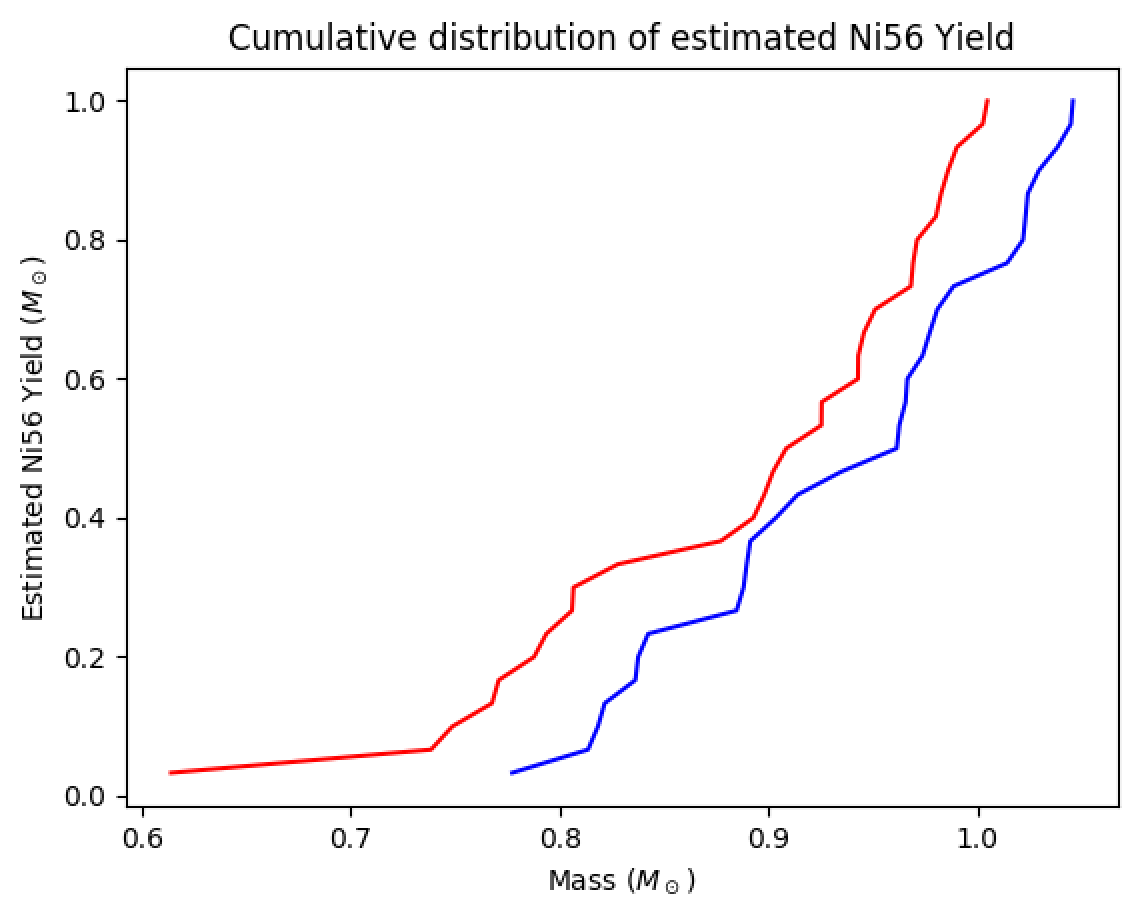
\includegraphics[width=\columnwidth]{figures/ni56_yield_cum_dist.png}
\caption{\label{fig:cumdist}
A plot of the estimated Ni56 yield as a function of the final, burned mass
for all CO and Hybrid runs. The Hybrid model is shown in red, and the CO
model is shown in blue. As it is shown, the CO model has a higher final mass
then the Hybrid model. 
}
\end{figure}

\begin{figure}
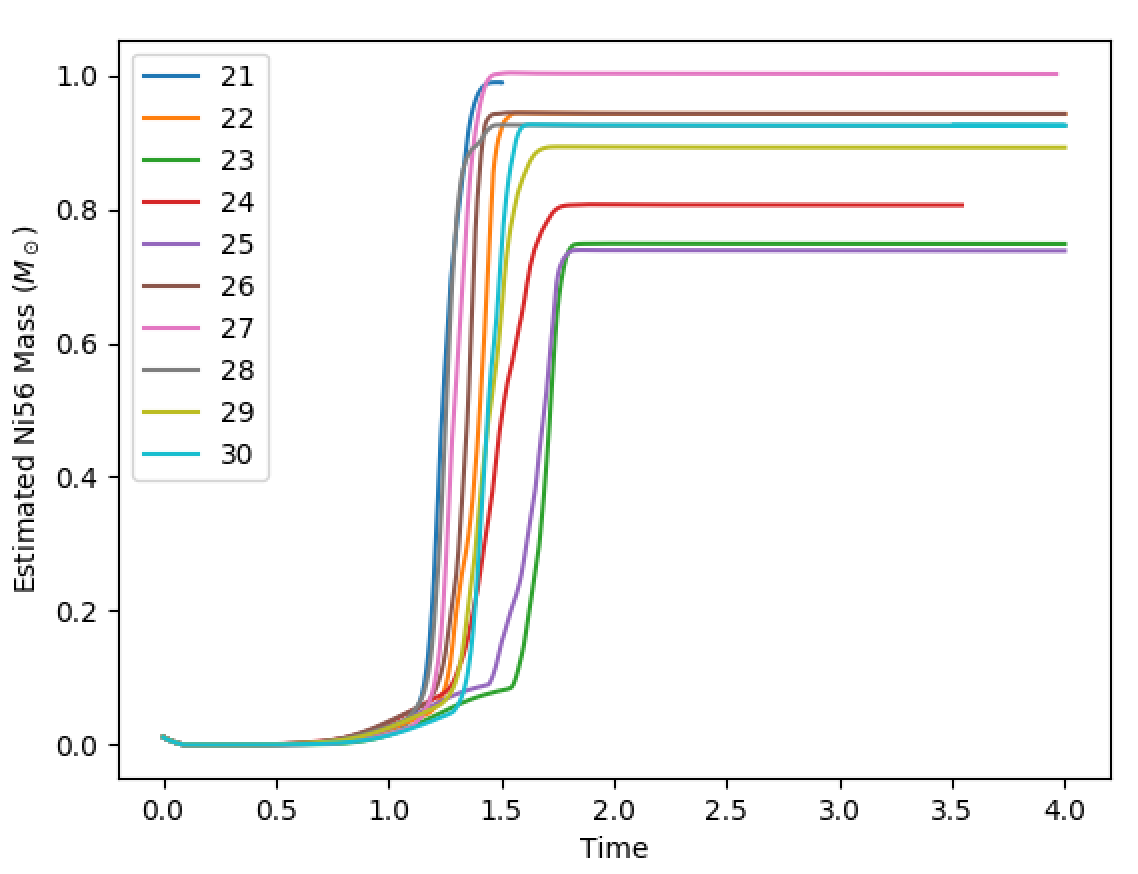
\includegraphics[width=\columnwidth]{figures/ni56_vs_time_hybrid.png}
\caption{\label{fig:nithybrid}
Estimated Ni56 mass for Hybrid Model
}
\end{figure}

\begin{figure}
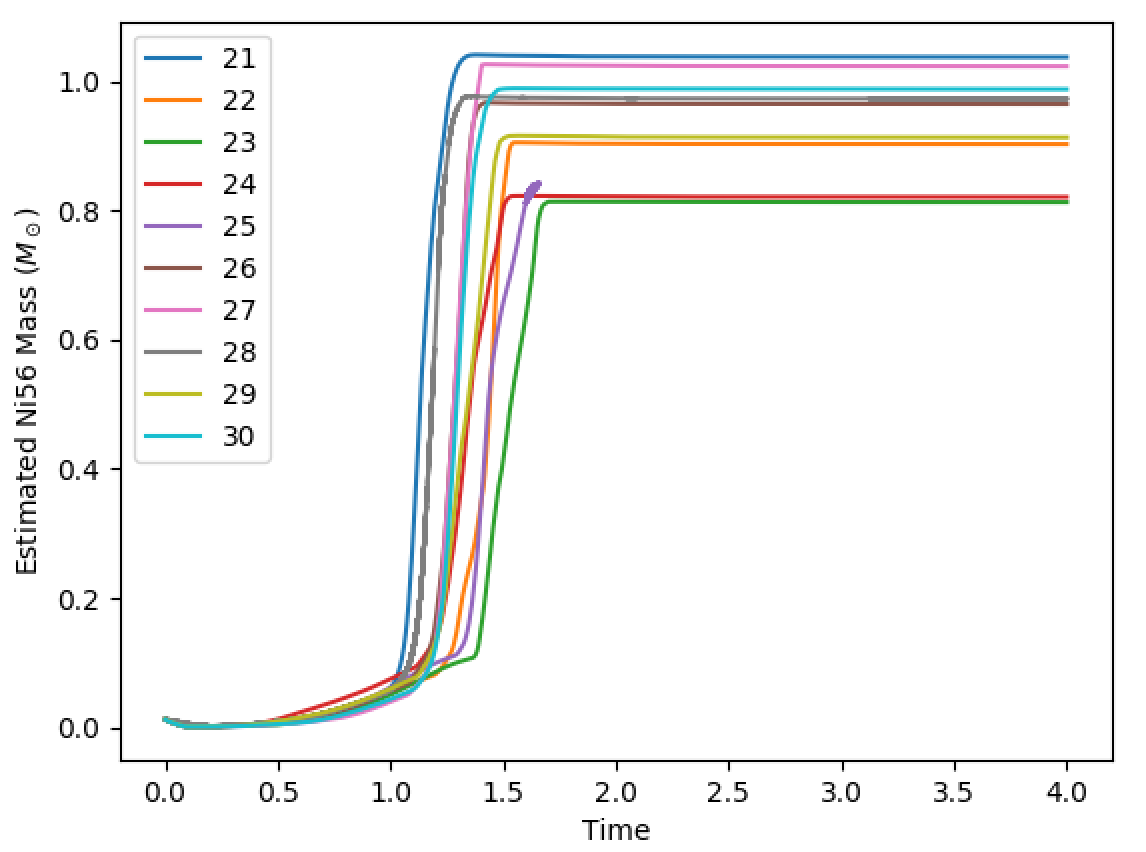
\includegraphics[width=\columnwidth]{figures/ni56_vs_time_CO.png}
\caption{\label{fig:nitco}
Estimated Ni56 mass for CO Model
}
\end{figure}

The figures show that the final Estimated Ni56 for the CO model is slightly
larger then the Hybrid model. Therefore, the CO produces more Ni56. The
Hybrid model has a larger range then the CO model. Also, on average, the CO
model reaches the DDT phase sooner then the Hybrid model. 

\begin{figure}
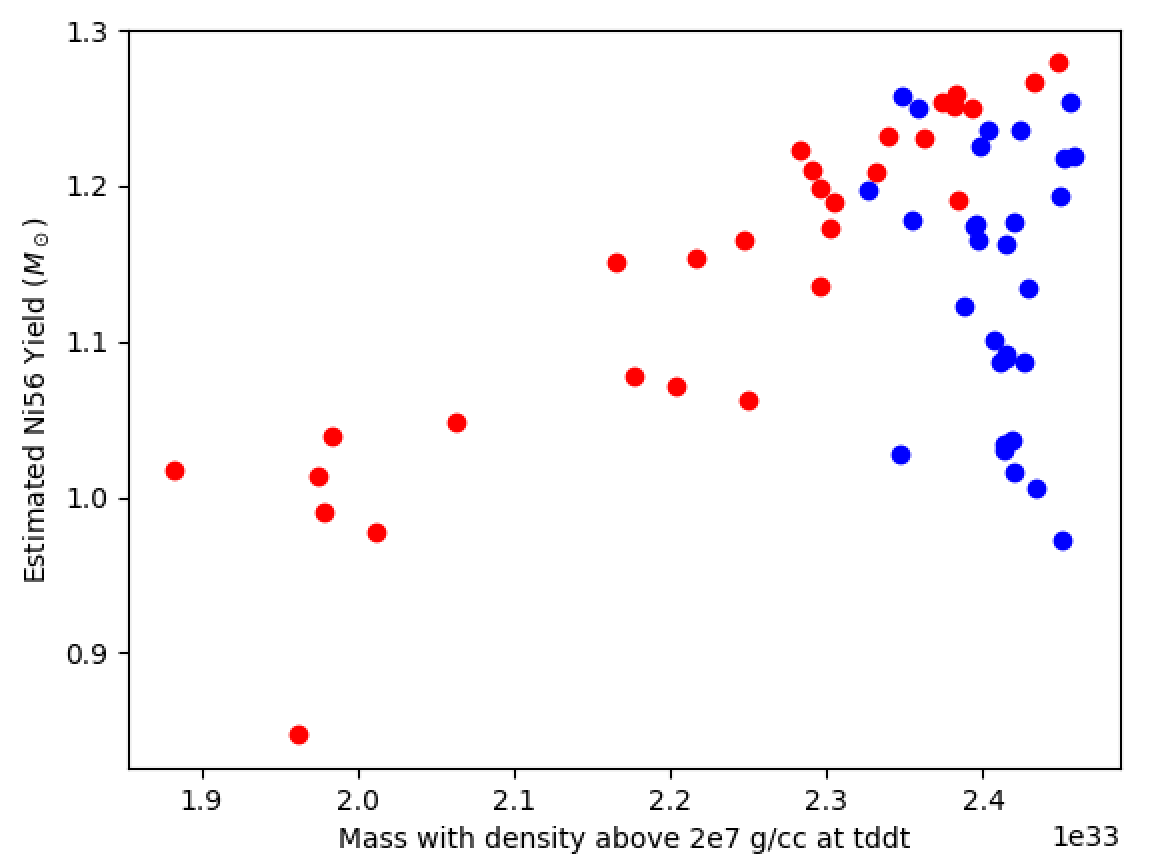
\includegraphics[width=\columnwidth]{figures/ni56_yield_vs_mass_at_high_dens.png}
\caption{\label{fig:masshighdens}
...
}
\end{figure}

\section{Discussion and Conclusion}







This work was supported in part by the Department of Energy under
grant DE-FG02-87ER40317. The software used in this work was in part
developed by the DOE-supported ASC/Alliances Center for Astrophysical
Thermonuclear Flashes at the University of Chicago. Results in this
paper were obtained using the high-performance computing system at the
Institute for Advanced Computational Science at Stony Brook
University.  other grants...

%%%%%%%%%%%%%%%%%%%%%%%%%%%%%%%%%%%%%%%%%%%%%%%%%%%%%%%%%%%%%%%%%%
% SOFTWARE
%% \software{
%%   FLASH \citep{Fryxetal00},
%%   CASTRO \citep{castro1},
%%   MESA \citep{mesa1},
%%   Matplotlib \citep{http://dx.doi.org/10.5281/zenodo.44579}
%% }

%%%%%%%%%%%%%%%%%%%%%%%%%%%%%%%%%%%%%%%%%%%%%%%%%%%%%%%%%%%%%%%%%%
\bibliography{master}


\end{document}

